\documentclass[../DS06.tex]{subfiles}
\graphicspath{{./figures/}}

% \subimport{/home/nora/Documents/Enseignement/Prepa/bpep/exercices/DS/lentille_magnetique/}{sujet.tex}

\begin{document}
\prblm[60]{Lentillage magnétique\ifcorrige{\textit{(D'après Banque PT 2017 et
  capes 2008)}}}

\enonce{
	La microscopie optique classique est limitée par la diffraction. Pour améliorer
	la résolution, on remplace les photons par des électrons de charge $q = -e$ et
	de masse $m$.
}

\QR{%
	Définir la diffraction. Donner, en argumentant, un ordre de grandeur de la résolution d'un microscope optique fonctionnant dans le visible.
}{%
	La diffraction est un phénomène ondulatoire se produisant lors de l'interaction d'une onde de longueur d'onde $\lambda$ avec un objet de dimension comparable à $\lambda$. La diffraction d'une onde engendre un éparpillement spatial de l'onde.

	La résolution d'un microscope optique est donc de l'ordre de la longueur d'onde du visible, soit $400 - \SI{800}{\nano\meter}$.
}

\partie{Aspect énergétique}
\enonce{
	Les électrons sont accélérés dans un canon à électrons
	(figure~\ref{fig:canon}) constitué de deux armatures planes et parallèles,
	distantes de $d = \SI{1}{\centi\meter}$ et séparées par du vide quasi-parfait.
	\begin{center}
		\input{./figures/canon.pdf_tex}
		\captionof{figure}{Schéma du canon à électrons.}
		\label{fig:canon}
	\end{center}
	On applique entre les armatures une tension positive $U = V_1-V_2$.  On suppose que le champ électrique $\vv{E}$ entre les armatures est uniforme.
}

\QR{%
	Représenter le champ électrique $\vv{E}$ entre les armatures. Sur quelle armature les électrons doivent-ils être émis sachant que leur vitesse initiale est nulle~? Exprimer la force électrique exercée sur l'électron en fonction de $E_0 = ||\vv{E}||$, $e$ et $\vv{u_z}$.
}{%
	Le champ électrique est orienté selon les potentiels décroissants, donc $\boxed{\vv{E} = -E_0\vv{u_z}}$.

	La force électrique s'exerçant sur l'électron s'écrit $\vv{F_e} = -e\vv{E} = eE_0\vv{u_z}$. Cette force est orientée selon $+\vv{u_z}$, donc les électrons doivent être \xul{émis depuis l'armature 2.}
	\begin{center}
		\input{./figures/canoncorr.pdf_tex}
	\end{center}
}

\QR{%
	Définir l'énergie potentielle électrique $E_p(z)$ de l'électron situé à la distance $z$ de l'armature 2 en fonction notamment du potentiel $V(z)$. Établir l'expression de $\vv{E}$ en fonction notamment de $U$.
}{%
	Par définition $E_p(z) = -eV(z)$. De plus, $\vv {F_e} = -\vv{\text{grad}}
		E_p$. On projette selon $\vv{u_z}$ :
	\eq{
		\dv{E_p}{z} = -eE_0
		\qdonc
		E_p(z) = -eE_0z+\text{cste}
	}

	En regardant entre $z = 0$ et $z = d$, on obtient
	\eq{
		E_p(z = d)-E_p(z = 0) = -e(V(z = d)-V(z = 0)) = -eU
	}
	Or $E_p(z = d)-E_p(z = 0) = -eE_0d$, d'où $E_0 = U/d$, donc $\boxed{\vv{E} = -\dfrac{U}{d}\vv{u_z}}$.
}

\enonce{
	On donne les valeurs numériques approchées :
	\eq{
		\cfrac{e}{m}\approx \SI{2e11}{S.I.}\qet \cfrac{h}{m}\approx \SI{7e-4}{S.I.},
	}
	où $h$ est la constante de Planck intervenant à la question~\ref{Q:planck}.
}

\QR{%
	Exprimer la vitesse $v$ atteinte par les électrons lorsqu'ils arrivent sur l'armature opposée, en fonction de $U$, $e$ et $m$. Calculer $v$ sachant que $U = \SI{1e5}{\volt}$. Commenter l'ordre de grandeur obtenu.
}{%
	L'électron, assimilable à un point matériel $M$ de masse $m$, est étudié dans
	le référentiel du laboratoire supposé galiléen. Il n'est soumis qu'à la force
	électrique (on néglige le poids) qui est une force conservative. Donc $E_m =
		cste$.

	On exprime l'énergie mécanique en $z = 0$ et en $z = d$ :
	\eq{
		E_m(z = 0) = -eV(z = 0)\quad ;\quad E_m(z = d) = -eV(z = d)+\cfrac{1}{2}mv^2
	}

	Comme $U = V(z = d)-V(z = 0)$, on en déduit $\boxed{v =
			\sqrt{\cfrac{2eU}{m}}}$.

	L'application numérique donne $\boxed{v = \SI{2e8}{\meter\cdot\second^{-1}}}$, donc la particule est relativiste.
}

\QR{\label{Q:planck}

	On donne la relation de de Broglie définissant la longueur d'onde d'une
	particule quantique : $p = h/\lambda$, avec $p$ la quantité de mouvement de la
	particule. Calculer la longueur d'onde $\lambda$ associée aux électrons ainsi
	accélérés. On utilisera ici la définition de la quantité de mouvement dans
	l'hypothèse d'une particule non-relativiste. On peut montrer qu'en considérant
	la particule comme étant relativiste, on aboutit à une longueur d'onde du même
	ordre de grandeur.
}{%
	Pour une particule non-relativiste, $p = mv$, donc $\boxed{\lambda =
			\SI{3,5e-12}{\meter}}$.
}


\partie{Déflecteur magnétique}
\enonce{
	Le rôle d'un déflecteur magnétique est simplement de dévier le faisceau
	d'électrons.

	On suppose qu'un électron de vitesse $\vv{v_0}$ arrive dans une zone où règne
	un champ magnétique uniforme $\vv{B}$ perpendiculaire au vecteur vitesse. Il
	n'y a plus de champ électrique.
}

\QR{%
	Justifier le fait que le mouvement de l'électron est uniforme.
}{%
	L'électron est soumis uniquement à la partie magnétique de la force de Lorentz
	$\vv{F_m} = -e\vv{v}\wedge\vv{B}$.

	D'après le théorème de la puissance cinétique $\dv{E_c}{t} =
		\vv{F_m}\cdot\vv{v}$.

	Par propriété du produit vectoriel $\vv{F_m}\bot \vv{v}$, donc
	$\vv{F_m}\cdot\vv{v} = 0$.

	On en déduit que $E_c = cste$, soit $v = ||\vv{v}|| = cste$. Le mouvement est
	uniforme.
}

\QR{%
	On admet que la trajectoire est circulaire. Tracer cette trajectoire, en faisant clairement apparaitre les vecteurs $\vv{v_0}$ et $\vv{B}$. Placer le centre $C$ de la trajectoire circulaire, ainsi que la base polaire $(\vv{u_r},\vv{u_\th})$ de centre $C$. L'axe de référence pour l'angle $\th$ sera pris parallèle à $\vv{v_0}$ et passant par $C$.
}{%
	\begin{center}
		\input{./figures/circulaire.pdf_tex}
	\end{center}
}

\QR{%
	Déterminer l'expression du rayon $R$ du cercle décrit en fonction de $m$, $v_0 = ||\vv{v_0}||$, $e$ et $B$.
}{%
	On applique la loi de la quantité de mouvement avec $\vv{a} = -\cfrac{v_0^2}{R}\vv{u_r}$ pour un mouvement circulaire uniforme  : $-m\cfrac{v_0^2}{R}\vv{u_r} = -ev_0\vv{u_\th}\wedge B\vv{u_z} = -ev_0B\vv{u_r}$

	On projette sur $\vv{u_r}$ : $\boxed{R = \cfrac{mv_0}{eB}}$.
}


\partie{Lentille magnétique}
\enonce{
	Le contrôle de la focalisation du faisceau électronique dans le microscope électronique est possible en utilisant des lentilles magnétiques. On s'intéresse ici à une lentille magnétique, modélisée par une bobine de $N$ tours confondus, circulaires de rayon $a$, de centre $O$, d'axe $Oz$ et parcourue par un courant permanent $I$. Cette bobine est obtenue par l'enroulement d'un fil électrique.

	Un point $M$ de l'espace sera repéré par ses coordonnées cylindriques $(r, \th, z)$ d'axe $Oz$ et de centre~$O$.

	En considérant les symétries et les invariances du bobinage, on peut justifier que le champ magnétique est indépendant de $\th$ et ne possède pas de composante orthoradiale. On peut alors écrire :
	\eq{
		\vv{B}(M) = B_r(r,z)\er+B_z(r,z)\ez
	}

	En pratique, le faisceau électronique passe dans le domaine $r\ll a$. Dans ce cas, on peut se contenter d'une expression approchée du champ $\vv{B}$ au voisinage de l'axe $Oz$ :
	\eq{
		\vv{B}(M)\approx -\cfrac{r}{2}\,\dv{B_z(0,z)}{z}\er+B_z(0,z)\ez
	}
	avec $B_z(0,z) = \cfrac{B_0}{\left ( 1+\cfrac{z^2}{a^2} \right )^{3/2}}$ le champ magnétique sur l'axe $Oz$ et $B_0 = \cfrac{\mu_0NI}{2a}$ le champ magnétique en $O$.


	On place en un point $P$ de l'axe $Oz$, en amont de la lentille magnétique, une
	source ponctuelle d'électrons. On considère un électron émis depuis le point $P$
	avec une vitesse $\vv{v_0}$.

	On ajoute les hypothèses simplificatrices suivantes à l'étude :
	\begin{itemize}
		\item L'électron est supposé non relativiste.
		\item L'électron ne subit que la force magnétique due à la lentille.
		\item Le vecteur vitesse initial $\vv{v_0}$ en $P$ est dans le plan méridien
		      $\th = 0$ et forme un angle $\alpha$ avec l'axe~$Oz$.
		\item L'angle $\alpha$ est faible ($\alpha\ll 1$) et la trajectoire ultérieure
		      de l'électron reste dans le domaine~$r\ll a$.
	\end{itemize}
}

\QR{%
	Produire un schéma paramétré dans un plan contenant l'axe $Oz$, et comportant la bobine, la définition des coordonnées cylindriques de $M$ et la base locale associée, ainsi que le vecteur $\vv{v_0}$.
}{%
	\begin{center}
		\input{./figures/coordonnees.pdf_tex}
	\end{center}
}

\QR{%
	A quelle approximation d'optique une de ces hypothèses fait-elle penser~? On définira cette approximation et on précisera les conséquences.
}{%
	La dernière hypothèse fait penser aux conditions de Gauss consistant à ne considérer que des rayons paraxiaux (proches de l'axe optique et faiblement inclinés par rapport à celui-ci).

	Dans ces conditions, il y a stigmatisme et aplanétisme approchés.
}

\QR{%
	Déterminer l'ordre de grandeur de la valeur de champ magnétique à partir de laquelle on peut ne pas tenir compte du poids de l'électron dans l'étude de son mouvement. On supposera que l'ordre de grandeur de la vitesse de l'électron est \SI{1e8}{\meter\cdot\second^{-1}}. Conclure.
}{%
	L'ordre de grandeur de la force magnétique est $F_m = evB$. Le poids s'exprime $P = mg$. On veut que $P/F_m\ll 1$ :
	\eq{
		\cfrac{mg}{evB}\ll 1\quad \Leftrightarrow \quad B\gg \cfrac{mg}{ev}\approx \cfrac{ 10}{2\times 10^{11}\times 10^{8}} = \SI{5e-19}{\tesla}
	}

	Il faut donc que $B$ soit supérieur à \SI{5e-19}{\tesla}, ce qui est une valeur extrêmement faible. Donc il est raisonnable de négliger le poids.
}

\QR{%
	Exprimer l'accélération de $M$ en coordonnées cylindriques, puis montrer que sa composante orthoradiale peut être mise sous la forme $\dfrac{1}{r}\dv{}{t}\pac{r^2\tp}$.
}{%
	On donne la vitesse et l'accélération en coordonnées cylindriques :
	\eq{
		\vv{v} = \rp \er+r\tp\et+\zp \ez\quad ;\quad \vv{a} = (\rpp -r(\tp)^2)\er+(r\tpp+2\rp  \tp)\et+\zpp \ez
	}

	On remarque que l'accélération orthoradiale peut s'écrire sous la forme :

	\[
		\cfrac{1}{r}\dv{}{t}\left [r^2\dv{\th}{t}\right ] = \cfrac{1}{r}(2r\rp \tp+r^2\tpp) = 2\rp \tp+r\tpp
	\]

}

\QR{%
	En déduire les trois équations différentielles du mouvement, que l'on notera (1), (2) et (3) et qui correspondent respectivement à la projection du principe fondamental de la dynamique sur $\er$, $\et$ et $\ez$.
}{%
	On exprime  la force de Lorentz dans la base cylindrique :

	\[
		\vv{F_m} = -e\vv{v}\wedge\vv{B} = -e
		\begin{pmatrix}
			\rp  \\
			r\tp \\
			\zp
		\end{pmatrix}
		\wedge
		\begin{pmatrix}
			-\cfrac{r}{2}\,\dv{B_z(0,z)}{z} \\
			0                               \\
			B_z(0,z)
		\end{pmatrix} = -e
		\begin{pmatrix}
			r\tp B_z(0,z)                                    \\
			-\cfrac{r}{2}\,\dv{B_z(0,z)}{z}\zp -\rp B_z(0,z) \\
			-r\tp\left (-\cfrac{r}{2}\,\dv{B_z(0,z)}{z}\right)
		\end{pmatrix}
	\]

	En projetant la loi de la quantité de mouvement dans la base cylindrique, on obtient les équations :
	\begin{eqnarray}
		\dv[2]{r}{t}-r\left ( \dv{\th}{t} \right )^2& = &-\cfrac{e}{m}\,r\,\dv{\th}{t}B_z(0,z)\label{eq:1}\\
		\dv{}{t}\left [r^2\dv{\th}{t}\right ]& = &\cfrac{e}{m}\,r\left [\dv{r}{t}B_z(0,z)+\cfrac{r}{2}\,\dv{z}{t}\,\dv{B_z(0,z)}{z}  \right ]\label{eq:2}\\
		\dv[2]{z}{t}& = &-\cfrac{e}{2m}\,r^2\,\dv{\th}{t}\,\dv{B_z(0,z)}{z}\label{eq:3}
	\end{eqnarray}
}

\QR{%
	Démontrer, à l'aide de l'équation~(2), la relation $\dv{\th}{t} = \cfrac{e}{2m}B_z(0,z)$.
}{%
	Le second membre de l'équation~(2) peut s'écrire :
	\begin{eqnarray*}
		\cfrac{e}{2m}\,\dv{}{t}\left [ r^2B_z(0,z) \right ]& = &\cfrac{e}{2m}\left [ 2r\rp B_z(0,z)+r^2\zp  \dv{B_z(0,z)}{z} \right ]\\
		& = &\cfrac{e}{m}\,r\left [\dv{r}{t}B_z(0,z)+\cfrac{r}{2}\,\dv{z}{t}\,\dv{B_z(0,z)}{z}  \right ]
	\end{eqnarray*}

	Par intégration de l'équation~2, $r^2\dv{\th}{t} = \cfrac{e}{2m}\,r^2B_z(0,z) +cste$.

	Or à $t = 0$, $r = 0$, donc la constante est nulle. On en déduit $\boxed{\dv{\th}{t} = \cfrac{e}{2m}B_z(0,z)}$.
}

\QR{%
	L'équation~(3) présente un second membre en $r^2$ négligeable dans le cadre de cette étude (car d'ordre 2 en $r/a$). Que vaut alors $\dv{z}{t}$~? En déduire, en partant de l'équation~(1), que l'évolution radiale $r(z)$ de l'électron vérifie l'équation différentielle
	\begin{equation}
		\dv[2]{r}{z}+\cfrac{e^2}{4m^2v_0^2}rB_z^2(0,z) = 0\label{eq:rz}
	\end{equation}
}{%
	Par intégration de l'équation~3, $\boxed{\dv{z}{t} = \text{cste} =
			v_0\cos(\alpha)\approx v_0}$. Par l'équation~1, en remplaçant $\tp$ par son
	expression $\dfrac{e}{2m}B_z(0,z)$ :


	\[
		\rpp -r\cfrac{e^2}{4m^2}\,B^2_z(0,z) = -\cfrac{e}{m} r\times \cfrac{e}{2m}B_z(0,z)\times B_z(0,z)\quad\Leftrightarrow \quad \rpp +r\cfrac{e^2}{4m^2}B^2_z(0,z) = 0
	\]



	Or $\dv{r}{t} = \dv{r}{z}\cdot\dv{z}{t}\approx v_0\dv{r}{z}$.  On dérive à nouveau, et on obtient

	\[
		\dv[2]{r}{t}\approx v_0\dv[2]{r}{z}\dv{z}{t}\approx v_0^2\dv[2]{r}{z} .
	\]



	D'où l'expression donnée dans l'énoncé.
	\eq{
		\boxed{\dv[2]{r}{z}+\cfrac{e^2}{4m^2v_0^2}rB_z^2(0,z) = 0}
	}
}


\QR{%
	On propose sur les figures~\ref{fig:tracer1} et~\ref{fig:tracer2} deux familles de tracés de fonctions $r(z)$ partant d'un point d'annulation avec un angle de départ $\alpha$ variable. Quelle figure représente effectivement un champ de solutions possible de l'équation~\ref{eq:rz} (on justifiera la réponse)~? Le système étudié joue-t-il bien son
	rôle attendu~?
	\smallbreak
	\begin{isd}
		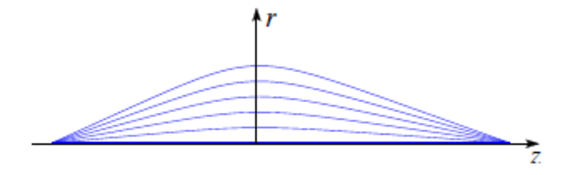
\includegraphics[width=.8\linewidth]{lentille1}
		\captionof{figure}{Proposition 1 de $r(z)$.}
		\label{fig:tracer1}
		\tcblower
		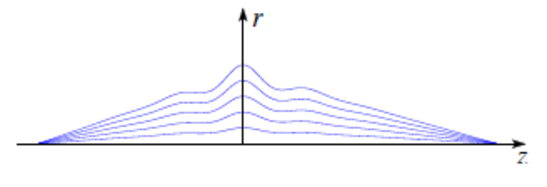
\includegraphics[width=.8\linewidth]{lentille2}
		\captionof{figure}{Proposition 2 de $r(z)$.}
		\label{fig:tracer2}
	\end{isd}
}{%
  D'après l'équation~4, $\boxed{\dv[2]{r}{z}<0}$, donc la courbe $r(z)$ est
  forcément \xul{concave}. Cette constatation est en accord avec la figure
  de gauche.

  On constate que les courbes $r(z)$  s'annulent en un point de l'axe $Oz$, avec
  $z>0$. Ce point $P'$ est le conjugué du point $P$. Donc le système joue bien
  le rôle d'une lentille.

}

\enonce{
	\begin{isd}
		On ajoute à présent l'hypothèse de lentille mince, c'est-à-dire que le champ magnétique du bobinage n'intervient que sur une zone faible d'épaisseur comprise entre deux plans $\Pi$ et $\Pi'$, de positions $-z_0$ et $z_0$ avec $z_0\ll OP$ (figure~\ref{fig:schemalentille}).

		Dans ces conditions, on peut montrer que la distance focale est approximativement donnée par
		\eq{
			f' = \cfrac{32m^2v_0^2}{3\pi ae^2B_0^2}
		}
		\tcblower
		\begin{center}
			\input{./figures/schemalentille.pdf_tex}
			\label{fig:schemalentille}
		\end{center}
	\end{isd}
}

\enonce{
	Dans ce cadre, on peut toujours écrire que
	\eq{
		\dv{\th}{t} = \cfrac{e}{2m}B_z(0,z)
	}

	et l'équation différentielle sur le mouvement radial $r(z)$ est utilisable sous la forme approchée
	\eq{
		\dv[2]{r}{z}\approx -\cfrac{e^2}{4m^2v_0^2}\,r_0B_z^2(0,z)
	}
	où $r_0$ est une valeur approchée de $r(z)$ (à l'ordre zéro en $r/a$) entre les plans $\Pi$ et $\Pi'$.
}
\QR{%
	Pourquoi la trajectoire d'un électron seul est forcément rectiligne en dehors de la zone de champ magnétique ?
}{%
	En dehors de la zone de champ magnétique, l'électron n'est soumis à aucune force. Donc d'après le principe d'inertie, il est animé d'un mouvement de translation rectiligne uniforme.
}

\QR{%
	Exprimer l'angle d'incidence $\alpha$ de l'électron en fonction de $r_0$ et de la distance algébrique $\obarr{OP}$.
}{%
	$\tan(\alpha) = -\cfrac{r_0}{\obarr{OP}}\approx \alpha$ (attention $\alpha>0$ et $\obarr{OP}<0$)
}

\QR{%
On note $P'$ le point de focalisation du rayon électronique, issu de la lentille, sur l'axe $Oz$ et on pose $\alpha'$ l'angle d'émergence de la zone magnétique tel que $\alpha '\approx -\cfrac{r_0}{\obarr{OP'}}$.

Préciser sur une figure l'angle $\alpha'$ et son orientation. Montrer que le système vérifie une loi de conjugaison de Descartes de lentille mince de centre $O$ et de focale $f'$ avec
\eq{
	\cfrac{1}{f'} = \cfrac{e^2}{4m^2v_0^2}\int_{-z_0}^{+z_0}B_z^2(0,z)\dd z
}

On rappelle la relation de conjugaison de Descartes $\cfrac{1}{\obarr{OA'}}-\cfrac{1}{\obarr{OA}} = \cfrac{1}{f'}$ avec $A'$ le point image conjugué du point objet $A$ à travers une lentille de centre optique $O$ et de focale image $f'$.
}{%
L'angle $\alpha'$ est l'angle entre l'axe $Oz$ et le rayon émergent. $\alpha'<0$, il est orienté dans le sens horaire.

Par définition $\tan(\alpha) = \dv{r}{z}(-z_0)$ et $\tan(\alpha') = \dv{r}{z}(z_0)$.

Les points $P$ et $P'$ étant conjugués, d'après la relation de conjugaison : $\cfrac{1}{\obarr{OP'}}-\cfrac{1}{\obarr{OP}} = \cfrac{1}{f'}$

\eq{
	\int_{-z_0}^{z_0}\dv[2]{r}{z}\dd z = \dv{r}{z}(z_0)-\dv{r}{z}(-z_0) = \alpha'-\alpha = -r_0\left (\cfrac{1}{\obarr{OP'}}-\cfrac{1}{\obarr{OP}}\right )
}

Or $\displaystyle \int_{-z_0}^{z_0}\dv[2]{r}{z}\dd z = -\cfrac{e^2r_0}{4m^2v_0^2}\int_{-z_0}^{+z_0}B_z^2(0,z)\dd z$. On en déduit
{\small $$-r_0\left (\cfrac{1}{\obarr{OP'}}-\cfrac{1}{\obarr{OP}}\right ) = -\cfrac{e^2r_0}{4m^2v_0^2}\int_{-z_0}^{+z_0}B_z^2(0,z)dz\quad \Leftrightarrow \quad \cfrac{1}{\obarr{OP'}}-\cfrac{1}{\obarr{OP}} = \cfrac{e^2}{4m^2v_0^2}\int_{-z_0}^{+z_0}B_z^2(0,z)dz$$}

On pose alors la distance focale
$\displaystyle\cfrac{1}{f'} = \cfrac{e^2}{4m^2v_0^2}\int_{-z_0}^{+z_0}B_z^2(0,z)\dd z$
}

\QR{%
	Montrer que, pendant le passage de l'électron dans la zone de champ magnétique, l'électron ne reste pas dans un même plan méridien et qu'il y a un angle de rotation $\Delta \th$ autour de l'axe $Oz$ de la trajectoire de l'électron qui vaut
	\eq{
		\Delta \th = \cfrac{e}{2mv_0}\int_{-z_0}^{z_0}B_z(0,z)\dd z
	}
}{%
	$\dv{\th}{t} = \dv{\th}{z}\,\dv{z}{t}\approx \dv{\th}{z}v_0$, donc $\dv{\th}{z} = \cfrac{1}{v_0}\dv{\th}{t} = \cfrac{e}{2mv_0}B_z(0,z)$.

	On intègre par rapport à $z$ :
	\eq{
		\Delta \th =\int_{-z_0}^{z_0}\dv{\th}{z}\,\dd z = \cfrac{e}{2mv_0}\int_{-z_0}^{z_0}B_z(0,z)\dd z
	}

}

\enonce{
	Dans le cas de la spire, les intégrales pouvant être étendues de $-\infty$ à  $+\infty$, un calcul non demandé donne
	\eq{
		\Delta \th = \cfrac{aeB_0}{mv_0}
	}
}

\QR{%
	Quel est le signe de $f'$~? Conclure.
}{%
	$f'>0$, donc la lentille est convergente.
}

\QR{%
	Sur quels paramètres peut-on jouer pour réduire $f'$ à tension accélératrice $U$ fixée~?
}{%
	Pour diminuer $f'$, il faut augmenter $aB_0^2 = \cfrac{N^2I^2}{a}$. On peut augmenter l'intensité $I$, ou diminuer le rayon $a$ des spires.
}

\QR{%
	On donne $B_0 = \SI{1.0}{\tesla}$, $a = \SI{1.0}{\milli\meter}$ et on choisit la tension accélératrice $U$ de sorte que ${v_0 = \SI{2.0e8}{\meter\cdot\second^{-1}}}$. Calculer $f'$ et $\Delta \th$.
}{%
	$f' = \SI{3,4}{\milli\meter}$ et $\Delta \th = \SI{1}{rad} = \SI{57}{\degree}$
}

\QR{%
	Les aberrations interviennent aussi avec une lentille magnétique mais l'aberration dite \og{}de charge d'espace\fg{} n'existe pas en optique classique. Quelle en est selon vous l'origine ? Pourquoi la réduction de cette aberration passe par l'utilisation de faisceaux électroniques peu denses ?
}{%
	Les électrons sont des particules chargées pouvant interagir entre eux par l'interaction électromagnétique. Ce n'est pas le cas des photons qui sont des particules non chargées.

	La répulsion entre les électrons rend la focalisation du faisceau électronique plus difficile. Cet effet est d'autant plus important que le faisceau électronique est dense.
}

\end{document}
